\documentclass{article}

\usepackage[paperwidth=6.5cm,paperheight=12cm, margin=0.2cm]{geometry}

\usepackage{tikz}
\usetikzlibrary{positioning, calc}
\tikzset{>=stealth}%\tikzset{>=latex}

\usepackage{pgfplots}
\pgfplotsset{compat=newest}
\pgfplotsset{samples=200}



\definecolor{green1}{RGB}{11,97,11}
\definecolor{green2}{RGB}{22,194,22}

\definecolor{path1}{RGB}{190,210,255}
\definecolor{path2}{RGB}{120,140,255}


\begin{document}
\centering


    
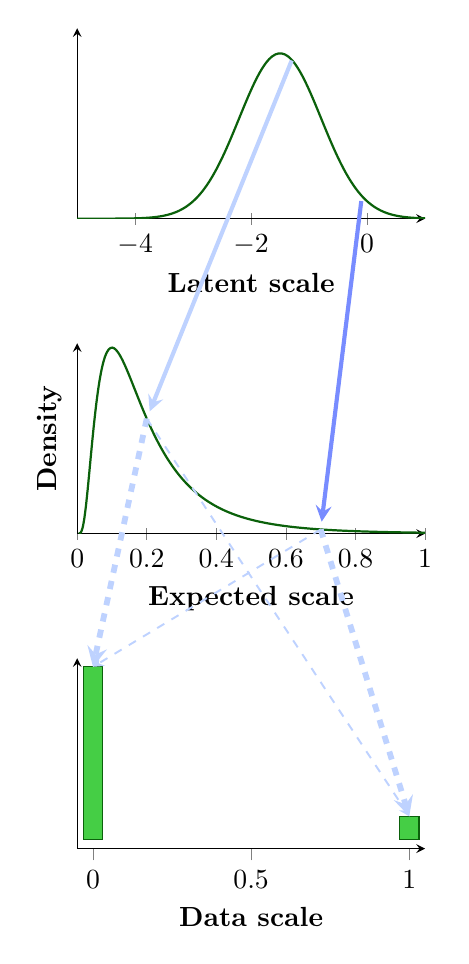
\begin{tikzpicture}

\def\hg{4cm}
\def\wg{6cm}

\begin{axis}[
width=\wg,
height=\hg,
at={(0cm,0cm)},
anchor= north west,
% enlargelimits=false,
axis x line=bottom,
axis y line=left,
ytick=\empty,
x tick label style={rotate=0,anchor=north},
xmin=-5,
xmax=1,
ymax=0.65,
domain=-7:4,
xlabel= \textbf{Latent scale}
]
 \addplot[green1, thick, smooth] {(1/(2*3.1415*0.5)^(1/2)) * e^( (-(x+1.5)^2) / (2*0.5) };
 %\addplot[green2, very thick, smooth] table[x=pxpx, y=pxpy, col sep=comma] {distrib.csv};
 \coordinate (lat1) at (axis cs:-1.3, 0.54);
 \coordinate (lat2) at (axis cs:-0.1, 0.06);
 \coordinate (forlab1) at (axis cs:0.6, -0.2);
\end{axis}

\begin{axis}[
width=\wg,
height=\hg,
at={(0cm,-\hg)},
anchor= north west,
axis x line=bottom,
axis y line=left,
ytick=\empty,
x tick label style={rotate=0,anchor=north},
xmin=0,
xmax=1,
ymax=0.45,
domain=0:1,
xlabel= \textbf{Expected scale},
ylabel= \textbf{Density}
]
 \addplot[green1, thick, smooth] {((1/(100*2*x*x*3.1415*0.5)^(1/2)) * e^( (-(ln(10*x)-0.5)^2) / (2*0.5) )};
 %\addplot[green2, very thick, smooth] table[x=pxpx, y=pxpy, col sep=comma] {distrib.csv};
 \coordinate (mod1) at (axis cs:0.2,0.2717);
 \coordinate (mod2) at (axis cs:0.7,0.0099);
 \coordinate (forlab2) at (axis cs:0.5, -0.15);
\end{axis}

\begin{axis}[
width=\wg,
height=\hg,
at={(0cm,-2*\hg)},
anchor= north west,
axis x line=bottom,
axis y line=left,
ytick=\empty,
xlabel =  \textbf{Data scale},
ybar,
enlargelimits=0.05,
bar width=7pt,
ymin=0
]
 %\addplot[green1, thick, smooth] {(1/(2*3.1415*1)) * e^( (-(x-2)^2) / (2*1) };
 %\addplot[green2, very thick, smooth] table[x=pxpx, y=pxpy, col sep=comma] {distrib.csv};
 %\begin{axis}[, ymax=55,ymin=0, minor y tick num = 3]
\addplot[green1, fill=green2!80!white] coordinates { (0, 0.88) (1, 0.12)};
  \coordinate (base3) at (axis cs:0,0);
  \coordinate (bar0) at (axis cs:0,0.88);
  \coordinate (bar1) at (axis cs:1,0.12);
  
\end{axis}

\draw[->, dashed, line width = 2.1pt, color= path1] (mod1)--(bar0);
\draw[->, dashed, line width = 0.7pt, color= path1] (mod1)--(bar1);

\draw[->, dashed, line width = 0.7pt, color= path1] (mod2)--(bar0);
\draw[->, dashed, line width = 2.1pt, color= path1] (mod2)--(bar1);

\draw[->, line width=1.5pt, color= path1, shorten >=0.1cm] (lat1)--(mod1);
\draw[->, line width=1.5pt, color= path2, shorten >=0.1cm] (lat2)--(mod2);


%\node (lab1) at (forlab1) {\textbf{Latent scale}};
%\node (lab2) at (forlab2) {\textbf{Expected scale}};

%%% REDRAW

    \end{tikzpicture}

\end{document}
